\documentclass{article}
\usepackage{mainPoly}

\title{Statistiques : Proportions, Évolutions}
\date{}
\author{Seconde 9}

\begin{document}
\maketitle

\section{Proportions et pourcentages}
\subsection{Populations}
\begin{tcolorbox}
\begin{definition}
En statistiques, on étudie des \textbf{populations}, c'est-à-dire des ensembles d'éléments appelés \textbf{individus}.  
\end{definition}
\end{tcolorbox}
\begin{example} 
Les ensembles suivants sont des populations pouvant faire l'objet d'études statistiques. 
\begin{itemize}
\item Le sport préféré des habitants de Villeneuve-Le-Roi;
\item Les initiales des élèves d'un lycée;
\item Le poids de pièces de métal fabriquées par une machine.
\item
\item 
\end{itemize}
\end{example}
\begin{tcolorbox}
\begin{definition}
On appelle \textbf{sous-population} d'une population $P$ une partie des individus de $P$.
\end{definition}
\end{tcolorbox}
\begin{example}
On donne des exemples de sous-population correspondant aux populations données ci-dessus:
\begin{itemize}
\item Les sports collectifs;
\item Les initiales commençant par des voyelles;
\item Les pièces pesant plus de $\qty{3,8}{\kilo\gram}$;
\item 
\item 
\end{itemize}
\end{example}
\begin{tcolorbox}
\begin{definition}
On conidère une population $P$ de $N$ individus et une sous-population $S$ de $P$ de $n$ individus. Alors la \textbf{proportion} de $S$ par rapport à $P$, notée $p$, est donné par
\begin{equation*}
p = \dfrac{n}{N}
\end{equation*}        
\end{definition}
\end{tcolorbox}
\begin{remark}
Pour obtenir la proportion d'une sous-population, on divise le nombre d'individus \textbf{concernés} par le nombre \textbf{total} d'individus. 
\end{remark}
\begin{example}
On vide une trousse de tous ses stylos (il y en a $15$), et on compte le nombre de stylos rouges (il y en a $3$). 
\begin{enumquestions}
\item Quelle est la population étudiée ? Et la sous-population ?
\item Quelle est la proportion de stylos rouges dans cette trousse ?
\end{enumquestions}

\emptybox{4cm}
\end{example}
\newpage

\subsection{Pourcentages}
\begin{tcolorbox}
\begin{remark}
Si l'on souhaite avoir la proportion $p$ sous la forme de \textbf{pourcentage}, il suffit de la multiplier par $100$.
\end{remark}
\end{tcolorbox}
\begin{example}
On considère les $56$ animaux d'un zoo : il y a $28$ lions, $12$ zèbres et $16$ alligators.
\begin{enumquestions}
\item Quelle est la population étudiée ?
\item Quelles sont les différentes sous-populations à l'étude ?
\item Donner la proportion de lions ($p_L$), de zèbres ($p_Z$) et d'alligators ($p_A$) \textbf{en pourcentage}.
\end{enumquestions}

\emptybox{4cm}
\end{example}

\begin{remark}
\hfill
\begin{itemize}
\item Si l'on connait la nombre total d'individus $N$ et la proportion $p$ de la sous-population $S$, alors on obtient le nombre d'individus $n$ de $S$ en faisant
\begin{equation*}
n = p \times N
\end{equation*}.
\item Autrement dit, prendre $p \%$ de $N$, c'est multiplier $N$ par $\dfrac{p}{100}$.
\item Si l'on connait $n$ et $p$, alors le nombre total d'individu $N$ est donné par
\begin{equation*}
N = \dfrac{n}{p}
\end{equation*}
\item Autrement dit, si $n$ représente $p \%$ de la population totale, alors le nombre total d'individu est donné par
\begin{equation*}
N = \dfrac{n}{p}100
\end{equation*}
\end{itemize}
\end{remark}
\begin{example}
\hfill
\begin{enumquestions}
\item Dans le lycée $A$, il y a $650$ élèves, dont $20\%$ de secondes. Combien y a-t-il de secondes ?
\item Il y a $50$ terminales dans le lycée $B$, et ils représentent $25\%$  de l'ensemble des élèves. Combien y a-t-il d'élèves au total dans le lycée $B$ ?
\end{enumquestions}

\emptybox{4cm}
\end{example}

\newpage
\subsection{Proportions de proportions}

\begin{example}
Dans un stade de $1600$ spectateurs, $40\%$ sont venus supporter l'équipe bleue. Parmi les supporteurs de l'équipe bleue, seul $60\%$ d'entre eux ont acheté une boisson. Combien de spectateurs sont à la fois supporteur de l'équipe bleue et ont acheté une boisson ?

\vspace*{0.2cm}
\emptybox{2cm}
\end{example}
\begin{proposition}
Soit $P$ une population, $S_1$ une sous-population de $P$, et $S_2$ une sous-population de $S_1$. Alors, $S_2$ est une sous-population de $P$.

De plus, si on note $p_1$ la proportion de $S_1$ par rapport à $P$ et $p_2$ la proportion de $S_2$ par rapport à $S_1$, alors la proportion de $S_2$ par rapport à $P$ est donnée par

\begin{equation*}
p = p_1 \times p_2
\end{equation*}
\end{proposition}
\begin{remark}
\begin{enumquestions}
\item La situation peut-être schématisée ainsi :

\begin{center}
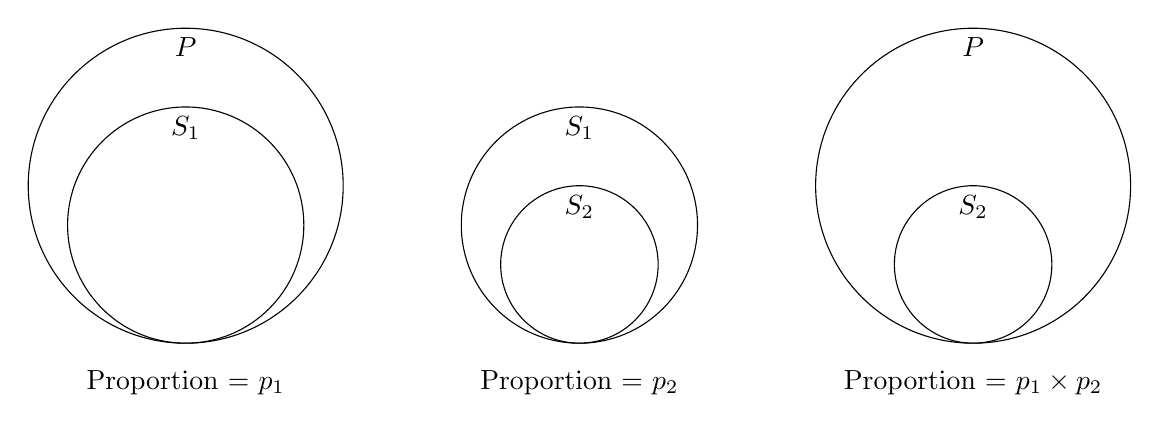
\begin{tikzpicture}
\draw (0,0) circle (2) (0,2) node[below]{$P$};
\draw (0,-0.5) circle (1.5) ++(0,1.5) node[below] {$S_1$};
\draw (0, -2.5) node {Proportion = $p_1$};
\begin{scope}[xshift = 5cm]
\draw (0,-0.5) circle (1.5) ++(0,1.5) node[below] {$S_1$};
\draw (0,-1) circle (1) ++(0,1) node[below] {$S_2$};
\draw (0, -2.5) node {Proportion = $p_2$};
\end{scope}
\begin{scope}[xshift = 10cm]
\draw (0,0) circle (2) (0,2) node[below]{$P$};
\draw (0,-1) circle (1) ++(0,1) node[below] {$S_2$};
\draw (0, -2.5) node {Proportion = $p_1 \times p_2$};
\end{scope}
\end{tikzpicture}
\end{center}
\item \textbf{Attention si les proportions sont données en pourcentages !} Dans ce cas, si l'on a $p_1 \%$ et $p_2\%$, la proportion de proportions correspondante est
\begin{equation*}
\dfrac{p_1}{100} \times \dfrac{p_2}{100}
\end{equation*} 
\end{enumquestions}
\end{remark}
\begin{example}
Dans un autre stade (\textbf{dont on ignore le nombre de spectateurs}), $40\%$ sont venus supporter l'équipe bleue. Parmi les supporteurs de l'équipe bleue, seul $60\%$ d'entre eux ont acheté une boisson. \textbf{Quelle est la proportion de spectateurs étant à la fois supporteur de l'équipe bleue et ayant acheté une boisson} ?

\vspace*{0.2cm}
\emptybox{3cm}
\end{example}
\newpage

\section{Évolution}
\subsection{Variation absolue, variation relative}
\textbf{On considère une quantité qui varie entre $V_d$ sa valeur de départ et $V_f$ sa valeur finale.}
\begin{tcolorbox}
\begin{definition}
\hfill
\begin{itemize}
\item La \textbf{variation absolue} de la quantité est donnée par $V_f - V_d$.
\item La \textbf{variation relative} de la quantité, aussi appelée \textbf{taux d'évolution}, est donnée par $\dfrac{V_f - V_d}{V_d}$.
\end{itemize}
\end{definition}
\end{tcolorbox}
\begin{remark}
\hfill
\begin{itemize}
\item La variation absolue possède la même unité que la quantité étudiée, tandis que la variation relative ne possède pas d'unité.
\item Quand la variation absolue ou relative est positive, c'est que la quantité a augmenté. Quand la variation absolue ou relative est négative, c'est que la quantité a diminué.
\item Le \textbf{taux d'évolution} peut être donné en pourcentage : il suffit de multiplier le taux d'évolution par $100$. 
\end{itemize}
\end{remark}
\begin{example}
Je possédais $V_d = 50€$ ce mois-ci, et je possèderai $V_f = 75€$ le mois prochain. Donner la variation absolue et le taux d'évolution concernant ce changement de budget.
\vspace*{0.5cm}

\emptybox{4cm}
\end{example}
\begin{proposition}
Soit $t = \dfrac{V_f - V_d}{V_d}$ le taux d'évolution. Alors $V_f = (1 + t)V_d$.

Autrement dit, il faut multiplier $V_d$ par $(1 + t)$ pour faire évoluer cette quantité vers $V_f$.
\end{proposition}
\begin{tcolorbox}
\begin{definition}
Le nombre $1 + t$, où $t$ est le taux d'évolution, est appelé \textbf{Coefficient Multiplicateur}.
\end{definition}
\end{tcolorbox}
\begin{example}
La température de la classe est initialement $V_d = \qty{20}{\degreeCelsius}$. Elle augmente de $25\%$. Calculer le coefficient multiplicateur associé et donner la température finale.
\vspace*{0.5cm}

\emptybox{3cm}
\end{example}
\newpage
\subsection{Évolutions successives}
\begin{example}
Le prix de l'électricité augmente de $5\%$ tous les ans pendant deux ans. De quel pourcentage a augmenté le prix de l'électricité après deux ans ?
\end{example}
\begin{center}
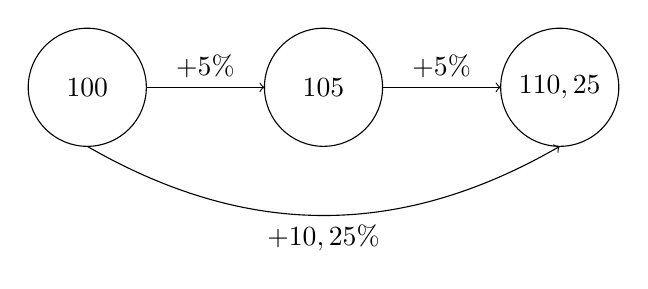
\begin{tikzpicture}
\draw (0,0) circle (0.75);
\draw (3,0) circle (0.75); 
\draw (6,0) circle (0.75);
\draw[->] (0.75,0) -- (2.25,0) node[midway,above] {$+5\%$};
\draw[->] (3.75,0) -- (5.25,0) node[midway,above] {$+5\%$};
\draw (0,0) node {$100$};
\draw (3,0) node {$105$};
\draw (6,0) node {$110,25$};
\draw[->] (0,-0.75) to[bend right] node[midway,below] {$+10,25\%$} (6,-0.75);
\end{tikzpicture}
\end{center}
\begin{tcolorbox}
\begin{proposition}
La succession de deux évolutions, respectivement de taux $t_1$ et $t_2$, a pour coefficient multiplicateur :
\begin{equation*}
CM_t = CM_1 \times CM_2 = (1 + t_1) \times (1 + t_2)
\end{equation*}
Alors, le taux d'évolution \textbf{global} associé à cette succession est donné par $t = CM_t - 1$.
\end{proposition}
\end{tcolorbox}
\begin{example}
Le prix du gaz, quant à lui, a augmenté de $t_1 = 20\%$ la première année puis a diminué de $t_2 = -40\%$ la deuxième année.
\begin{enumquestions}
\item Donner les coefficients multiplicateurs $CM_1$ et $CM_2$ associés à $t_1$ et à $t_2$.
\item En déduire le coefficient multiplicateur $CM_t$ de la succession d'évolutions.
\item En déduire le taux d'évolution global $t$.    
\end{enumquestions}
\vspace*{0.5cm}

\emptybox{3cm}
\end{example}
\newpage
\subsection{Évolution réciproque}
\begin{example}
Un article est soldé de $33\%$ en 2024. Mais, en 2025, on souhaite augmenter son prix d'un certain pourcentage afin d'obtenir son prix initial. Quel est ce pourcentage ?

\begin{center}
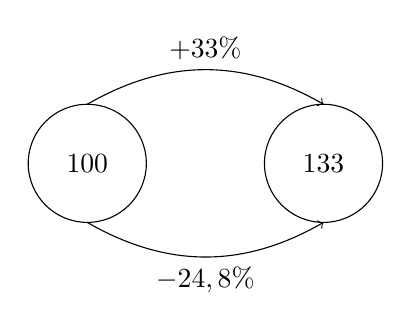
\begin{tikzpicture}
\draw (0,0) circle (0.75);
\draw (3,0) circle (0.75);
\draw (0,0) node {$100$};
\draw (3,0) node {$133$};
\draw[->] (0,0.75) to[bend left] node[midway,above] {$+33\%$} (3,0.75);
\draw[->] (0,-0.75) to[bend right] node[midway,below] {$-24,8\%$} (3,-0.75);
\end{tikzpicture}
\end{center}
\end{example}
\begin{tcolorbox}
\begin{proposition}
Soit un taux d'évolution $t$, décrivant l'évolution depuis une valeur $V_d$ vers une valeur $V_f$. Son coefficient multiplicateur est noté $CM$. 

Alors, pour calculer le taux de l'évolution de $V_f$ vers $V_d$, on calcule son coefficient multiplicateur
\begin{equation*}
CM_r = \dfrac{1}{CM}
\end{equation*}

Alors le taux d'évolution \textbf{réciproque} est donné par
\begin{equation*}
t_r = CM_r - 1
\end{equation*}
\end{proposition}
\end{tcolorbox}
\begin{example}
Un autre article est augmenté de $t = +60\%$. On se demande par quel pourcentage solder cet article pour qu'il retrouve son prix d'origine.
\begin{enumquestions}
\item Calculer le coefficient multiplicateur $CM$ associé à ce taux d'évolution.
\item En déduire le coefficient multiplicateur \textbf{réciproque} $CM_r$.
\item En déduire le taux d'évolution réciproque $t_r$.
\end{enumquestions}
\vspace*{0.5cm}

\emptybox{3cm}
\end{example}
\end{document}